%%%% utfpr-poster.tex, 2019/12/01
%%%% Copyright (C) 2018-2019 Luiz E. M. Lima (luizeduardomlima@gmail.com)
%%
%% This work may be distributed and/or modified under the conditions of the
%% LaTeX Project Public License, either version 1.3 of this license or (at your
%% option) any later version.
%% The latest version of this license is in
%%   http://www.latex-project.org/lppl.txt
%% and version 1.3 or later is part of all distributions of LaTeX version
%% 2005/12/01 or later.
%%
%% This work has the LPPL maintenance status `maintained'.
%%
%% The Current Maintainer of this work is Luiz E. M. Lima.
%%
%% This work consists of the files utfpr-poster.sty and utfpr-poster.tex.
%%
%% A brief description of this work is in readme.txt.

%% Detecção e aviso sobre comandos obsoletos
% \RequirePackage[l2tabu, orthodox]{nag}

%% Classe de documento e opções
\documentclass[%% Opções: [>] passada para pacotes
  final,%% Em oposição à de rascunho (draft) [>]
  english,%% Idioma secundário (penúltimo) [>]
]{beamer}

%% Pacotes utilizados
\usepackage[%% Opções: [>] passada para beamerposter
  Times   = false,%% Fontes Times (roman) e Arial (sans serif): true ou false
  BibURLs = false,%% Links de URLs nas referências: true ou false
  ABNTNum = none,%% Estilo numérico ABNT: none (AUTOR, ANO), dflt (1) e brkt [1]
  size    = custom,%% Tamanho de papel: a0, a1, a2, a3, a4 e custom [>]
  width   = 80,%% Largura de papel em centímetros (custom) [>]
  height  = 180,%% Altura de papel em centímetros (custom) [>]
  scale   = 1.43,%% Escala de fontes [>]
]{utfpr-poster}
\usepackage{blindtext}
\usepackage{multirow}
% \usepackage[english]{babel}
% \usepackage[square,numbers]{natbib}
% \bibliographystyle{abbrvnat}

%% Arquivo de referências
\addbibresource{utfpr-poster.bib}
\addbibresource{utfpr-poster.bib}
\addbibresource{utfpr-poster.bib}

%% Informações do documento
%%%% Título
\title{%
  COMBINING MULTIPLE TREE REARRANGEMENT OPERATORS\\ FOR EFFICIENT PARSIMONY INFERENCE USING\\ REINFORCEMENT LEARNING APPROACH%
}
%%%% Assunto
\subject{Scientific Research Conference 2023 - UET}
%%%% Autor(es)
\author{%
  Students: Dung Tien Huynh%
  \and Tuan Quoc Vu%
  \and Dung Viet Nguyen%
  \and\\Science Instructor: Dr. Diep Thi Hoang%
}
%%%% Instituição(ões) e e-mail(s)
\institute{%
  \showthe\font\affil{UNIVERSITY OF ENGINEERING AND TECHNOLOGY
}%
  \and{FACULTY OF INFORMATION TECHNOLOGY}%
  \and\email{21020007@vnu.edu.vn}%
  \sep\email{21020033@vnu.edu.vn}%
  \sep\email{21020043@vnu.edu.vn}%
  \sep\email{diepht@vnu.edu.vn}%
}
%%%% Data: comente para gerar a data atual
\date{}

%% Início do documento
\begin{document}
\setbeamertemplate{background} {

\includegraphics[width = \paperwidth, height = \paperheight]{Figuras/background.png}
}
% \setbeamertemplate{background} 
% {
% \includegraphics[width = \paperwidth, height = \paperheight]{Figuras/Picture1.jpg}
% }
\begin{frame}[t, fragile = singleslide]

\begin{columns}[t, onlytextwidth]%% Início do cabeçalho
%

\begin{column}{0.1\textwidth}
\begin{flushleft}

\includegraphics[width = \columnwidth]{./Logos/UET-logo.png}
\end{flushleft}
\end{column}
%
\begin{column}{0.8\textwidth}
\titlepage%
\end{column}
%
\begin{column}{0.1\textwidth}
\begin{flushright}

\includegraphics[width = \columnwidth]{./Logos/FIT-logo}%% Logomarca superior-direito
\end{flushright}
\end{column}
%
\end{columns}%% Fim do cabeçalho

\begin{columns}[t, onlytextwidth]
%
\begin{column}{0.49\textwidth}
\vspace{-0.9cm}
\begin{block}{INTRODUCTION}
\begin{itemize}
\item In bioinformatics, the phylogenetic tree is a fundamental concept that traces the evolutionary history of a group of species back to a common ancestor. This study specifically addresses the challenge of parsimony phylogenetic bootstrapping, which entails reconstructing the phylogenetic tree through analysis of biological sequences and gauging the reliability of the partitions within the tree.
\item As sequencing technology advances, researchers can generate vast amounts of data for phylogenetic analyses, making it essential to investigate more efficient techniques for phylogenetic bootstrapping.
\begin{figure}[!htb]
\label{fig:campuspontagrossa}
\centering%
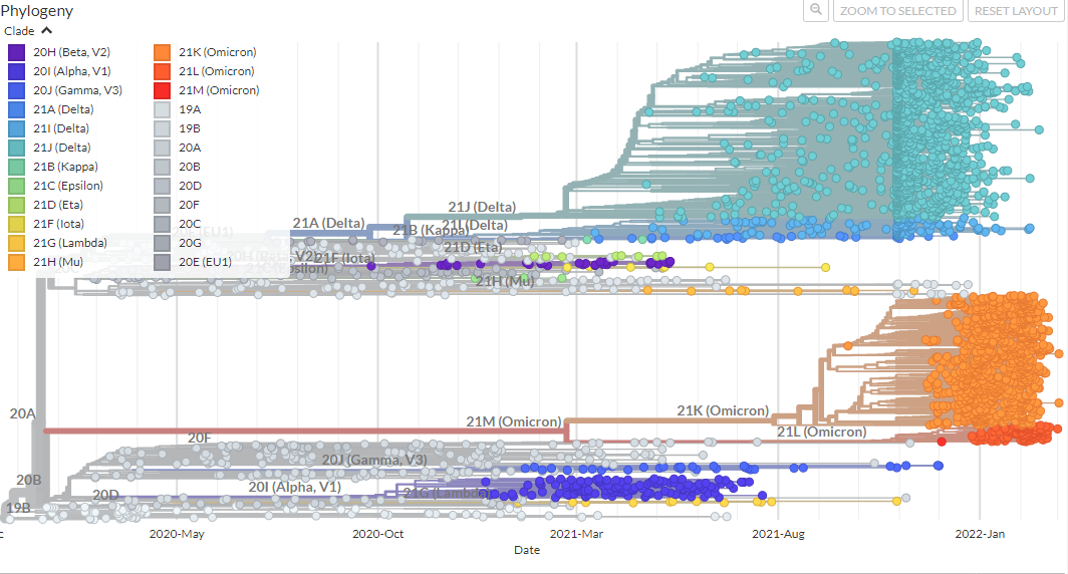
\includegraphics[width = 0.5\columnwidth]{./Figuras/covid2.png}
\caption{Phylogenetic tree of Sars-CoV-2 constructed from millions of samples.}%
\end{figure}
\item We aim to improve the efficiency of MPBoot \cite{Hoang2018}, a widely used method for parsimony bootstrapping, by integrating tree bisection and reconnection (TBR) transformation. Our MPBoot-TBR algorithm utilizes optimization techniques to search for TBR transformations and hill climbs using TBR, improving sampling efficiency. Additionally, we introduce the MPBoot-ACO algorithm, which uses ant colony optimization to combine hill climbing of three transformations, including TBR, to enhance program performance.
\end{itemize}

\begin{figure}[!htb]
\centering%
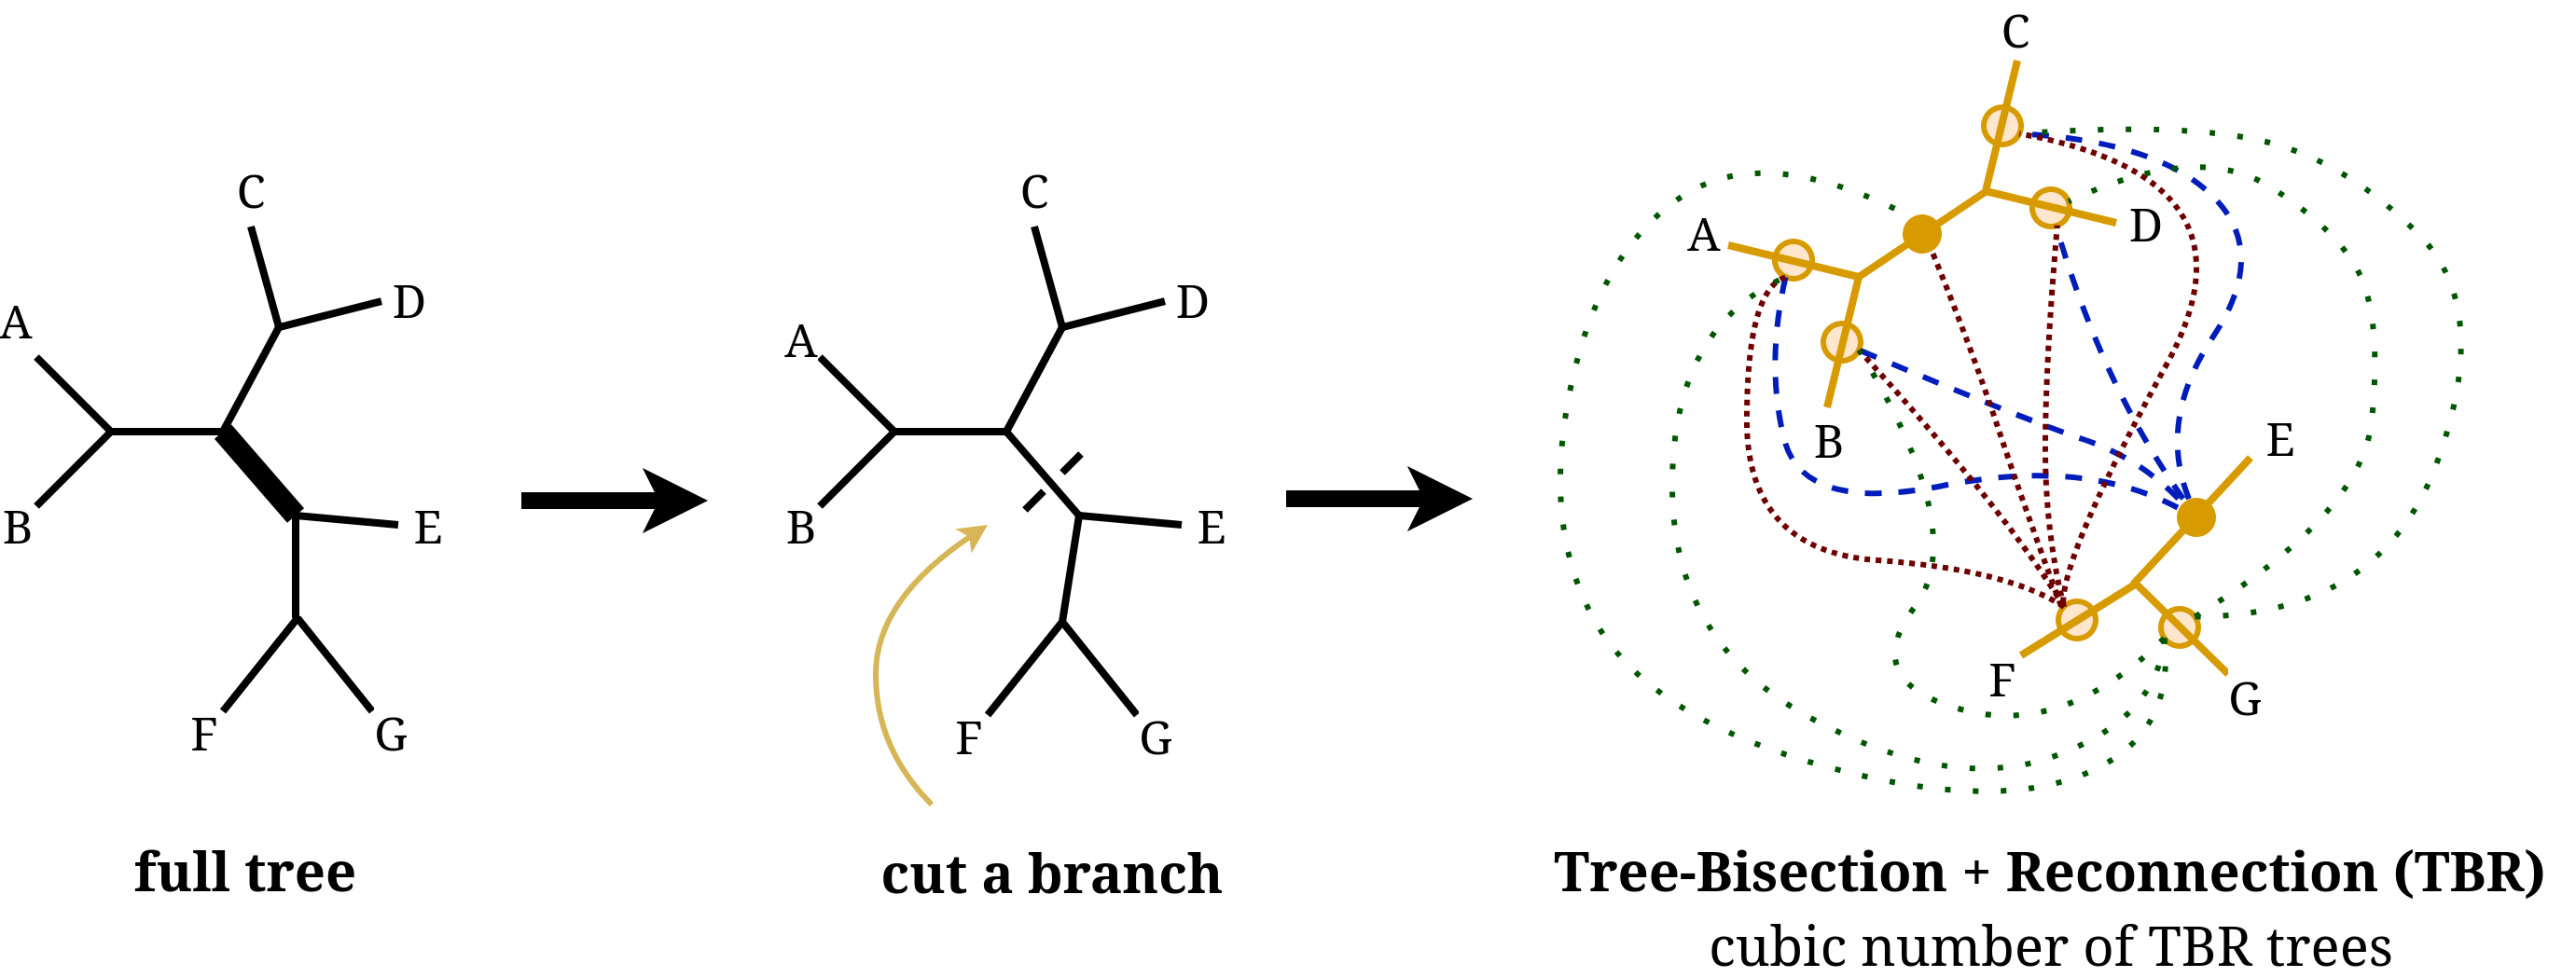
\includegraphics[width = 0.92\columnwidth]{./Figuras/TBR.drawio.png}
\caption{Tree bisection and reconnection (TBR) tree transformation.}%
\end{figure}

\end{block}
%
\end{column}
%
\begin{column}{0.48\textwidth}
\vspace{-0.9cm}
\begin{block}{ABOUT MPBOOT}

\begin{figure}[!htb]
\centering%
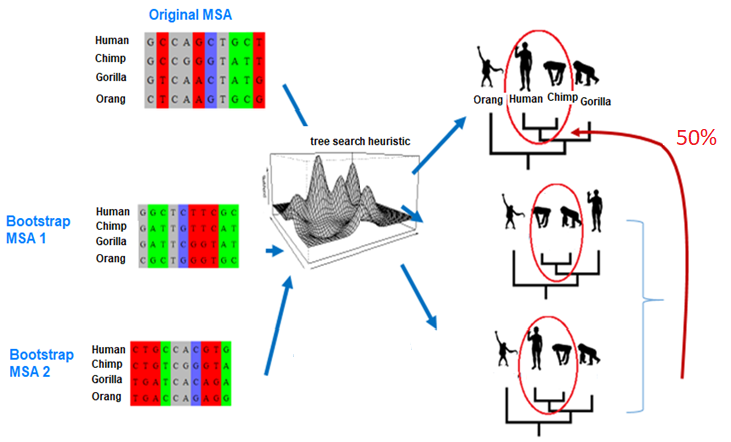
\includegraphics[width = 0.8\columnwidth]{./Figuras/mpboot.png}
\caption{Summarizing bootstrap results.}%
\end{figure}

\begin{itemize}
\item MPBoot speeds up over the standard bootstrap (SBS) \cite{10.2307/2408678} with its approximation method. Each bipartition's reliability is calculated by its frequency on the bootstrap tree set - the best trees on pseudoreplicates of the original multiple sequence alignment. Unlike SBS, MPBoot requires only one tree search on the original MSA since it applies resampling parsimony score (REPS) to reuse the original MP column scores for bootstrap MP scores. MPBoot approximates the bootstrap tree set once the original tree search completes.
\item MPBoot currently relies solely on SPR for tree rearrangement. Incorporating TBR, a more advanced operation, and combining it with NNI and SPR would potentially improve the MP tree and bootstrap tree set.
\end{itemize}

\begin{figure}[!htb]
\centering%
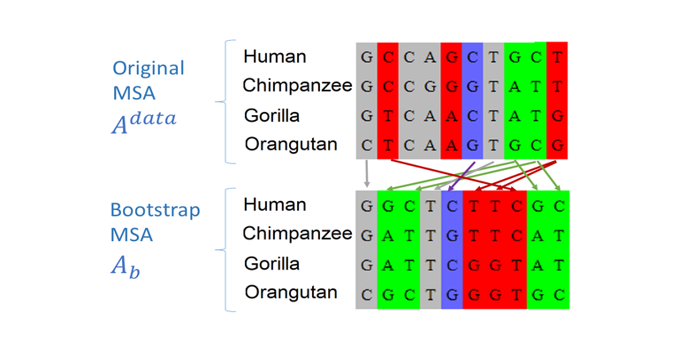
\includegraphics[width = 0.6\columnwidth]{./Figuras/REPS.png}
\caption{REPS: Resampling Estimated Parsimony Scores
.}%
\end{figure}

\end{block}
%
\end{column}
%
\end{columns}

\begin{columns}[t, onlytextwidth]
%
\begin{column}{\textwidth}
%
\begin{block}{PROPOSED METHOD 1: MPBoot-TBR}

\begin{columns}

\begin{column}{0.48\textwidth} 
\begin{figure}
\centering%
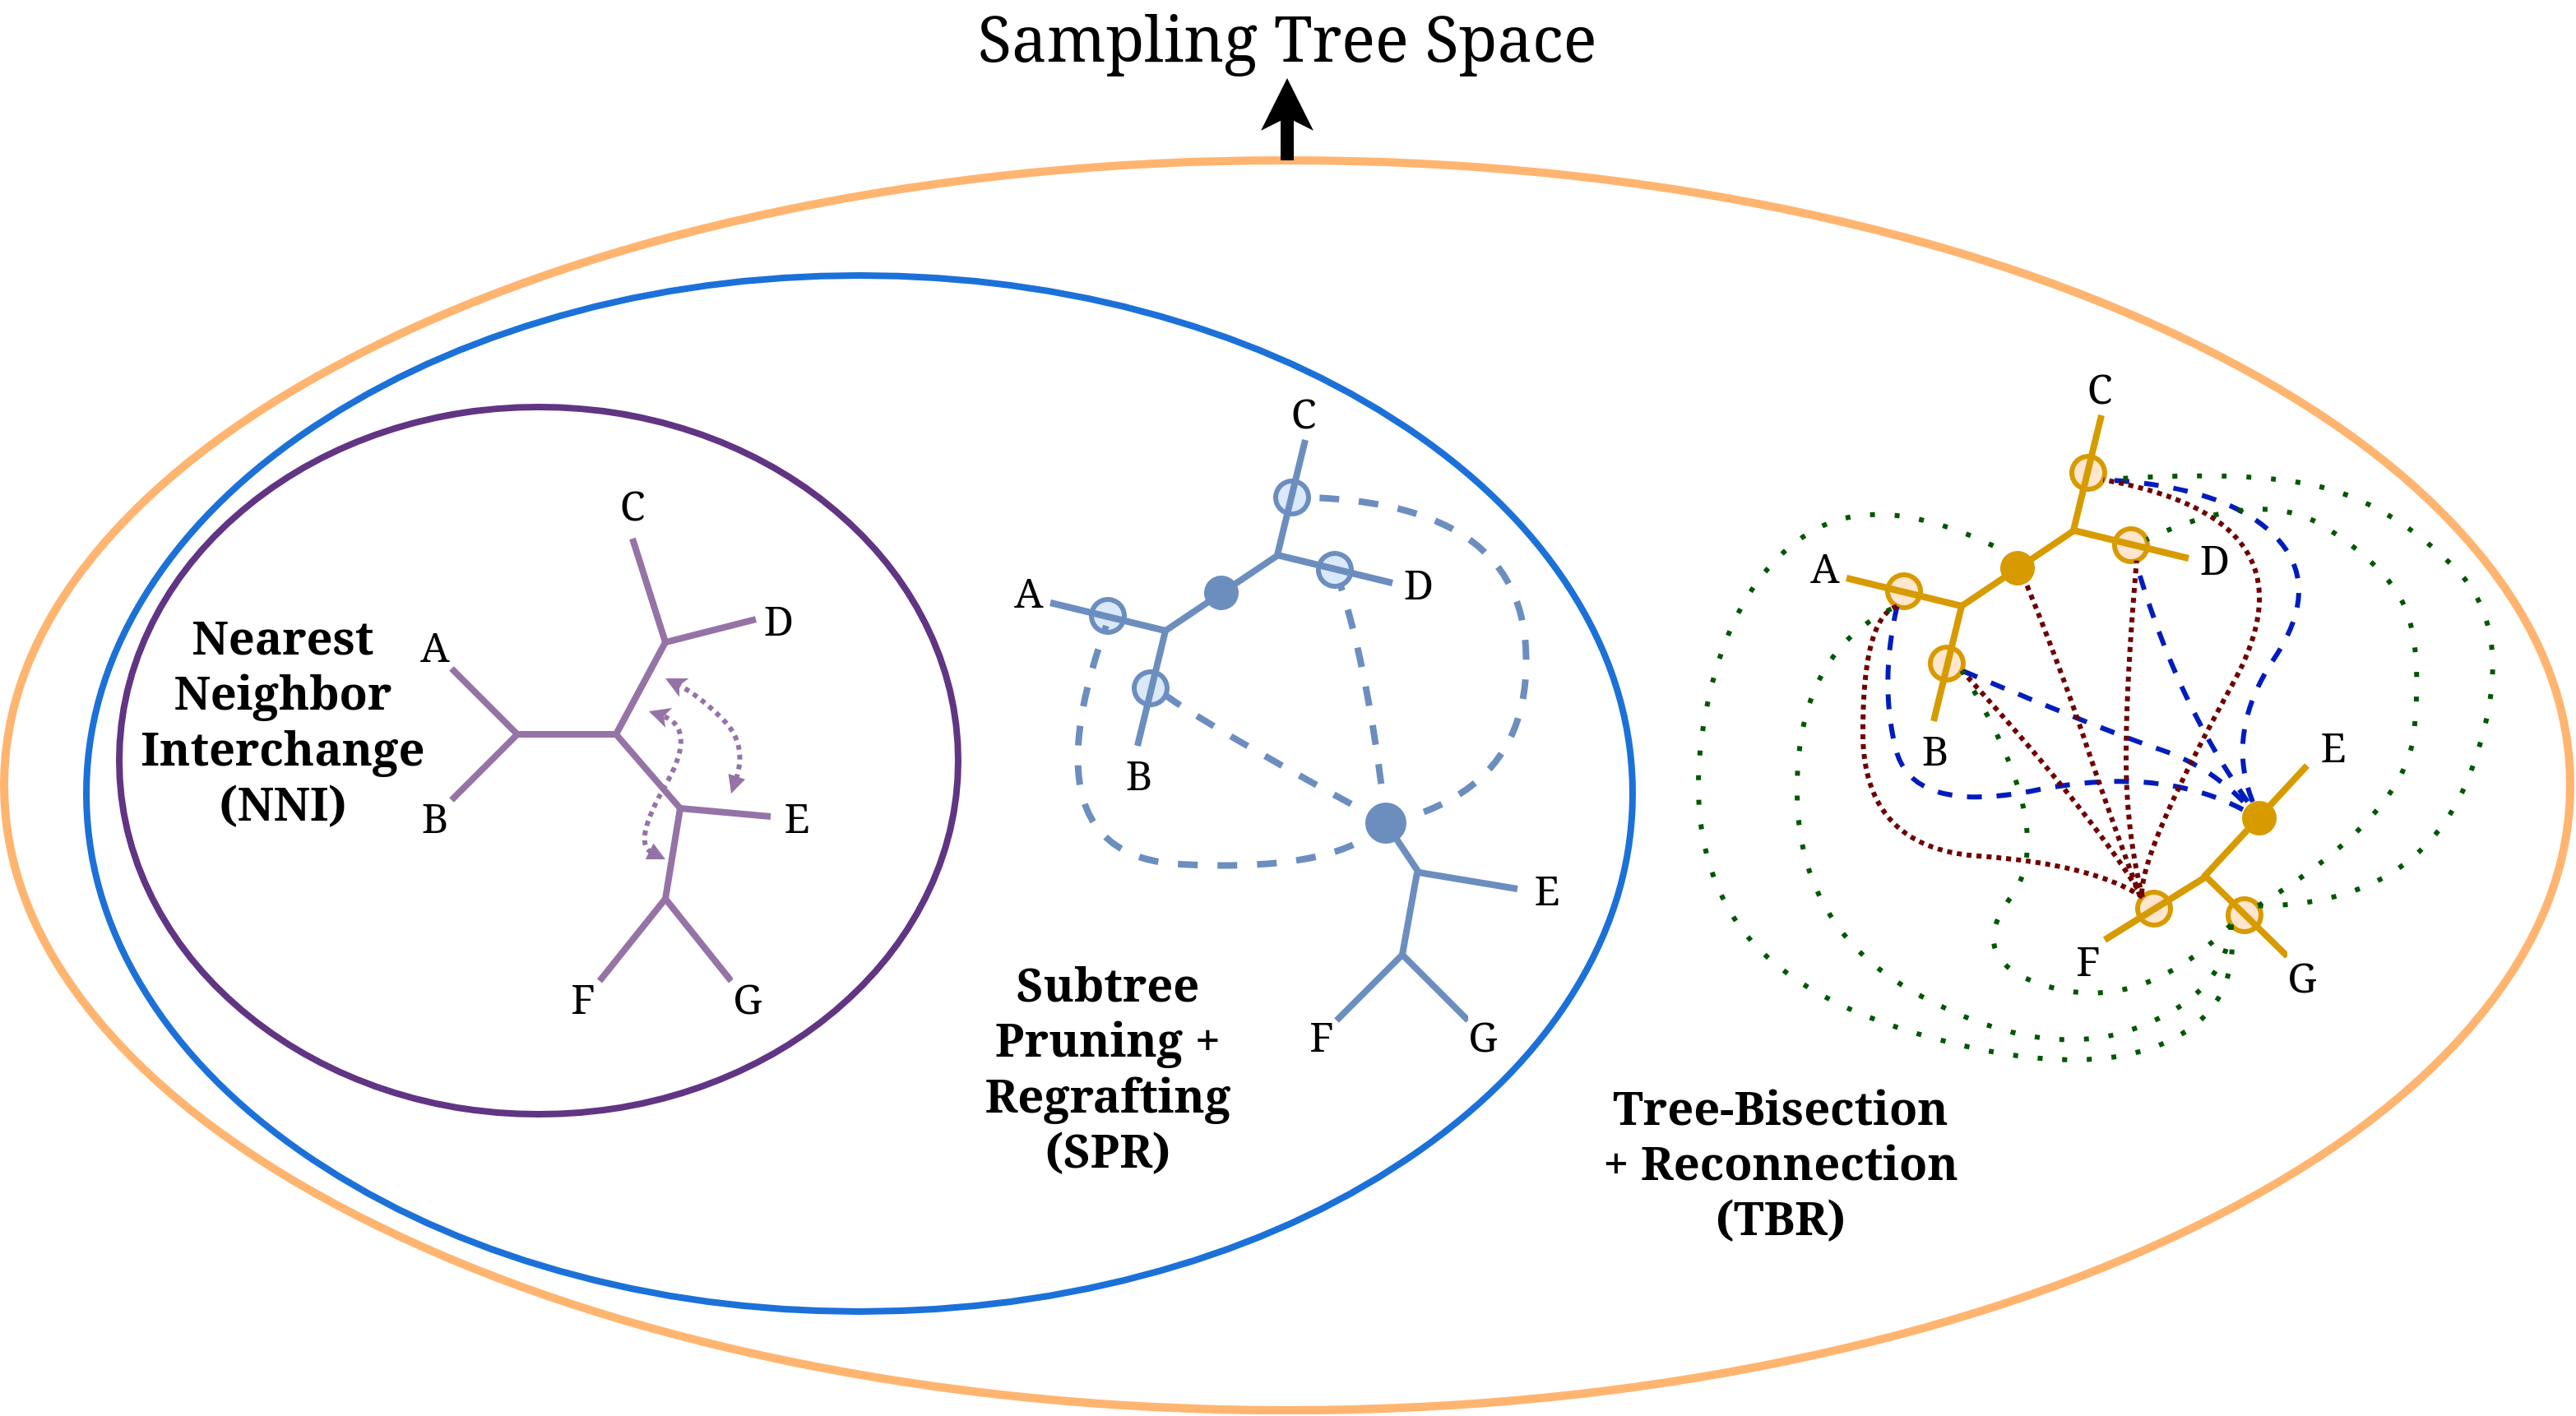
\includegraphics[width = 0.78\columnwidth]{./Figuras/3-operations.drawio.png}
\caption{Sampling tree space of NNI, SPR, and TBR transformation illustrated.}%
\end{figure}
Due to the enhanced tree search space, TBR is time-consuming. To address this, we suggest a method for faster TBR move evaluation that avoids the unnecessary recalculation of MP scores for unchanged subtrees. \\
\vspace{0.8cm}
\end{column} 

\begin{column}{0.45\textwidth}
\begin{figure}
\centering%
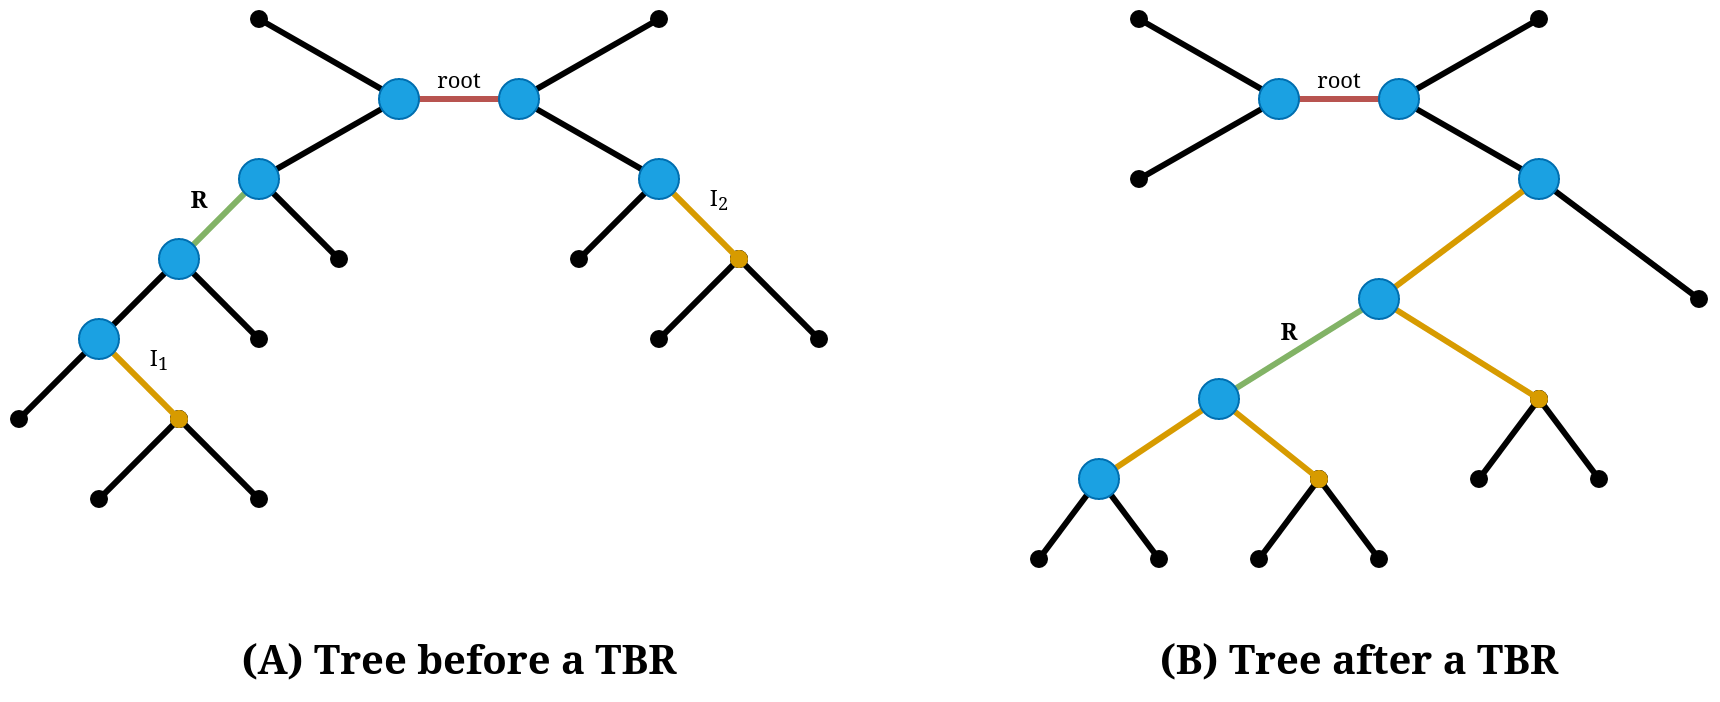
\includegraphics[width = 0.8\columnwidth]{./Figuras/tbr-recalculated-nodes.drawio.png}
\caption{Highlighted nodes indicate the nodes that require recalculation.}%
\end{figure}
\vspace{0.6cm}
MPBoot-TBR is proposed as a substitute for SPR hill-climbing, with two TBR search strategies: MPBoot-TBR-best and MPBoot-TBR-better. The search continues while MP score is improved, with unsuccessful iterations tracked to determine search termination.
\end{column}

\end{columns}
\end{block}

\begin{block}{PROPOSED METHOD 2: MPBoot-ACO}
\begin{columns}
\begin{column} {0.35\textwidth}
MPBoot-ACO is recommended as a better alternative to hill-climbing algorithms that only use SPR or TBR by combining ACO with NNI, SPR, and TBR operations. \\ 
\vspace{0.7cm}
The algorithm selects the most appropriate operation among NNI, SPR, and TBR, rather than the most intensive one, to maintain accuracy while improving computational speed. 
\end{column}
\begin{column} {0.57\textwidth}
\begin{figure}
\centering%
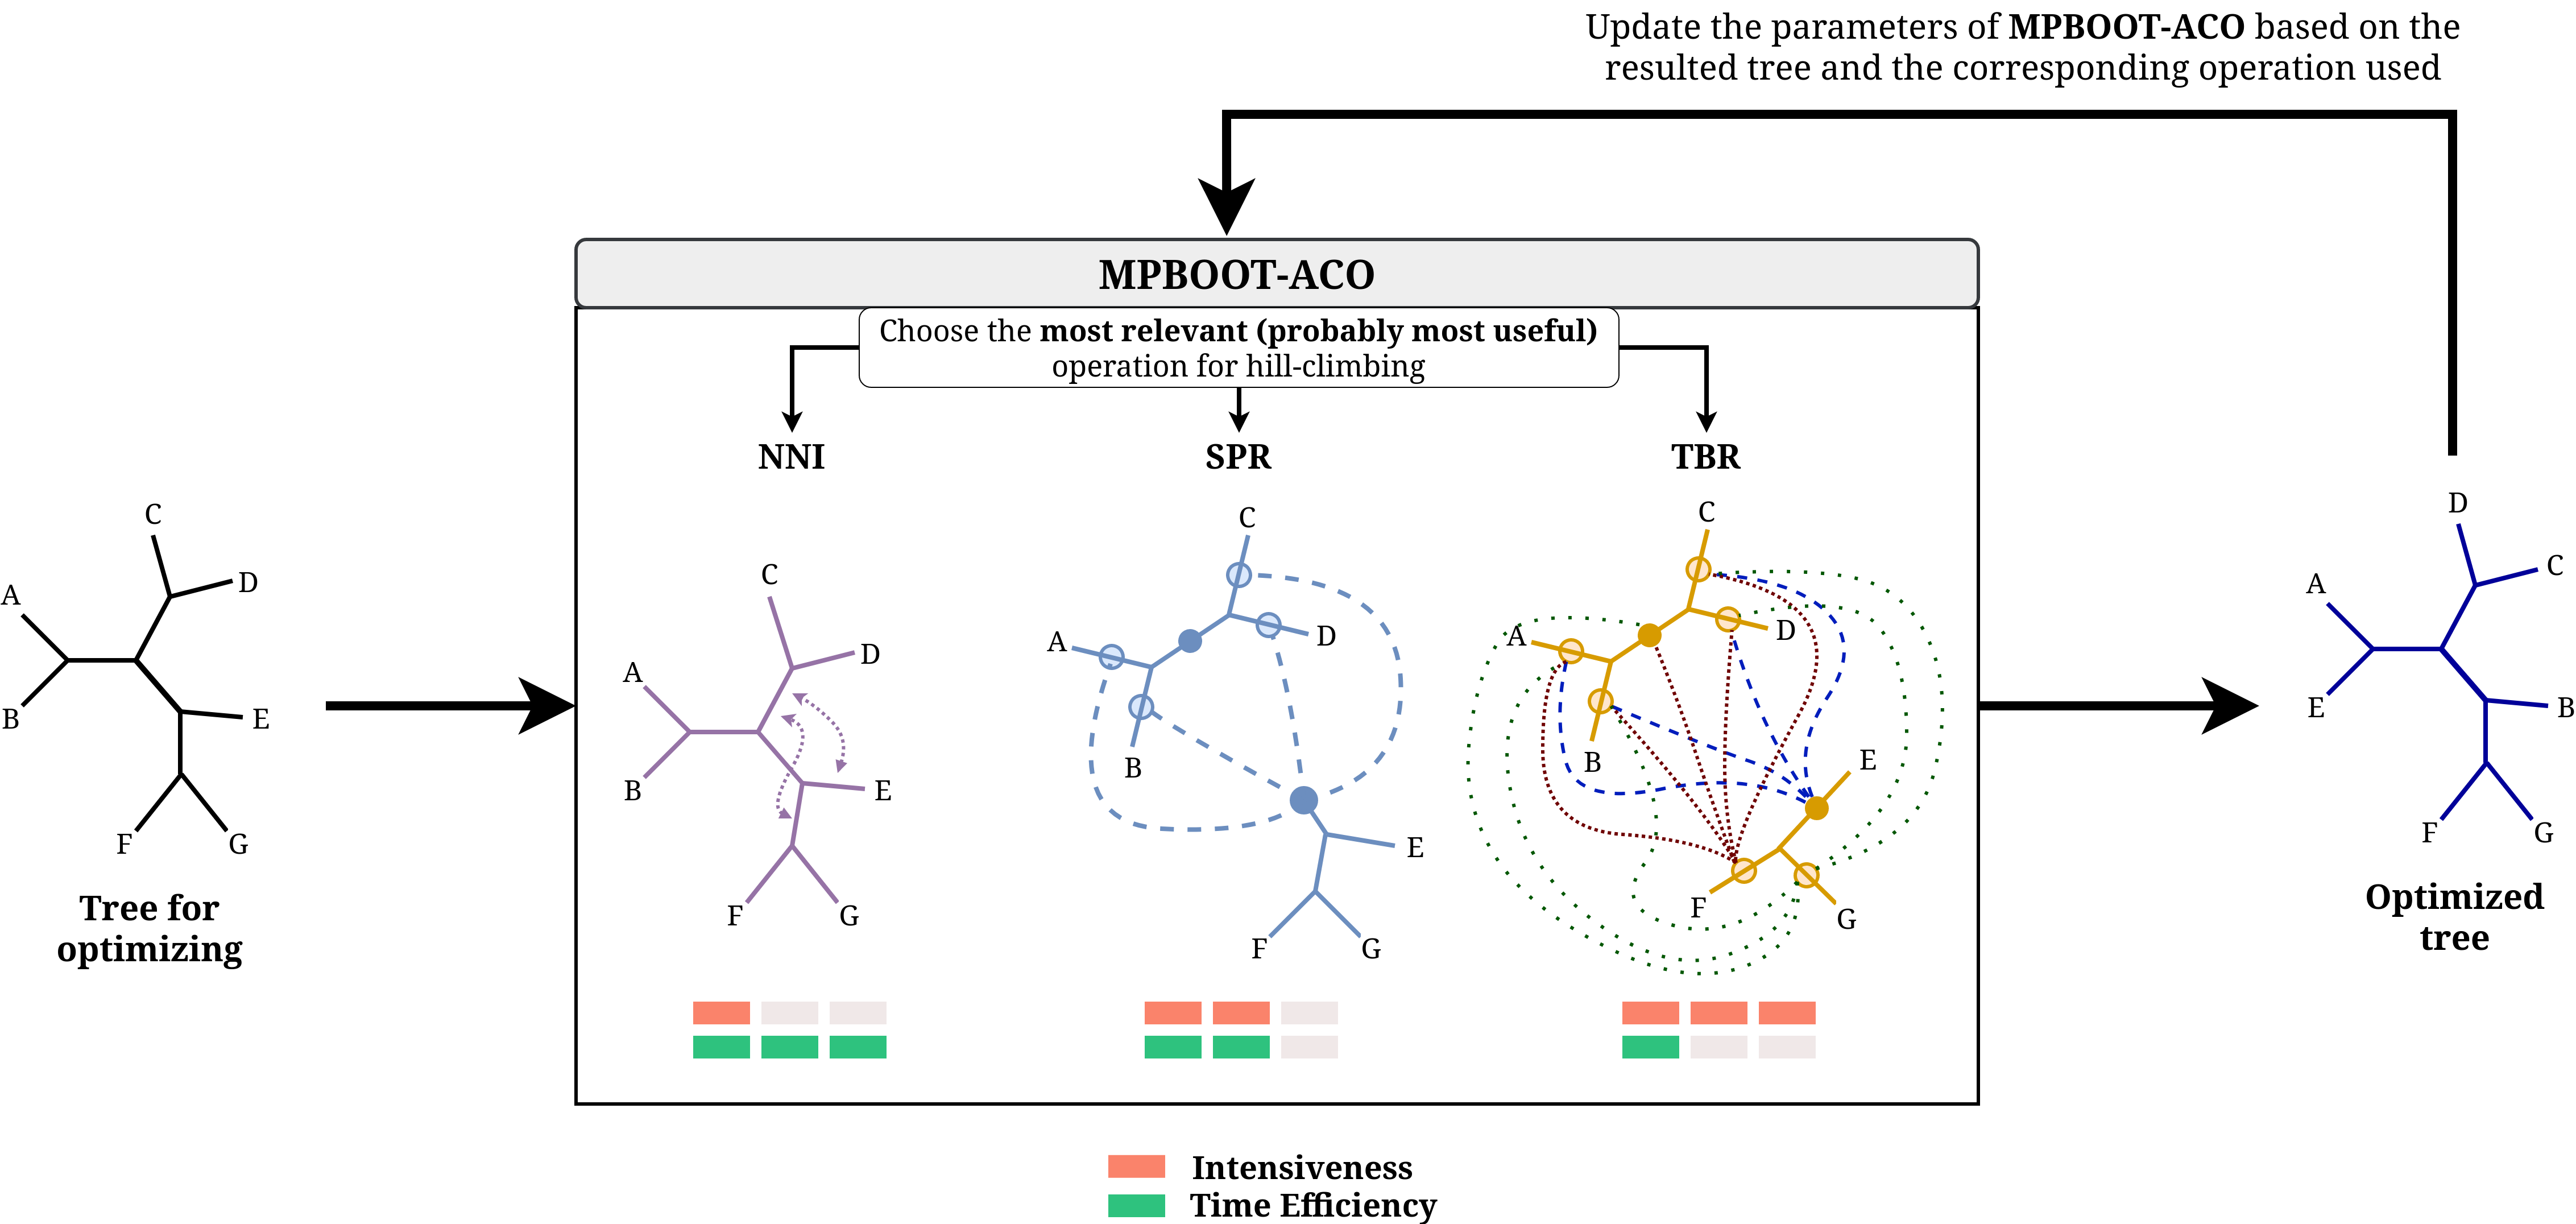
\includegraphics[width = 0.98\columnwidth]{./Figuras/MPBoot-ACO.drawio.png}
\caption{MPBoot-ACO algorithm.}%
\end{figure}
\end{column}
\end{columns}
\end{block}
\end{column}
\end{columns}

\begin{columns}[t, onlytextwidth]
%
\begin{column}{\textwidth}
%
\begin{block}{EXPERIMENTAL EVALUATION}
\begin{columns}

\begin{column}{0.48\textwidth}
\begin{itemize}

\item We compared four variations of MPBoot-TBR with the original MPBoot and also evaluated MPBoot-ACO against MPBoot-TBR-best (abbreviated as MPBoot-TBR) and the original MPBoot. The assessment was conducted on the high-performance computing system of VNU University of Engineering and Technology, using both biological and simulation data.
    \item We used MP Scores, Bootstrap Accuracy and Computational Time as evaluation metrics to compare proposed algorithms and the original algorithm.
\end{itemize}
\vspace{0.05cm}
\begin{table}
\centering%
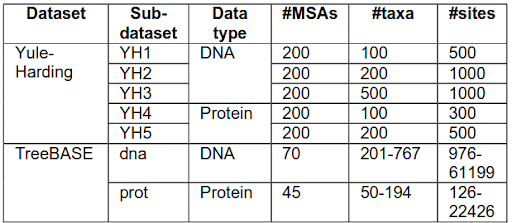
\includegraphics[width = 0.65\columnwidth]{./Figuras/datasets.png}
\caption{Summary of the datasets.}
\end{table}

% \item We use benchmark simulation datasets generated according to the Yule Harding model ~\cite{harding1971} and two real datasets: TreeBASE dataset \cite{citeulike:10413065} and SARS-CoV-2 dataset \cite{Wu2020}.
% \begin{table}[]
% \centering
% \caption{Summary of the datasets}
% \label{tab:table 1}
% \begin{tabular}{|l|l|l|l|l|l|}
% \hline
% Dataset                      & Sub-dataset   & Data type                                              & \#MSAs & \#sequences & \#sites   \\ \hline
% \multirow{5}{*}{YuleHarding} & YH1           & \multirow{3}{*}{DNA}                                   & 200    & 100         & 500       \\ \cline{2-2} \cline{4-6} 
%                              & YH2           &                                                        & 200    & 200         & 1000      \\ \cline{2-2} \cline{4-6} 
%                              & YH3           &                                                        & 200    & 500         & 1000      \\ \cline{2-6} 
%                              & YH4           & \multirow{2}{*}{Protein}                               & 200    & 100         & 300       \\ \cline{2-2} \cline{4-6} 
%                              & YH5           &                                                        & 200    & 200         & 500       \\ \hline
% \multirow{2}{*}{TreeBASE}    & TreeBASE-dna  & DNA                                                    & 70     & 200-767     & 976-61199 \\ \cline{2-6} 
%                              & TreeBASE-prot & Protein                                                & 45     & 50-194      & 126-22426 \\ \hline
% SARS-CoV-2                   &               & \begin{tabular}[c]{@{}l@{}}Whole\\ genome\end{tabular} & 1      & 3685        & 30462     \\ \hline
% \end{tabular}
% \end{table}



\end{column}
% \begin{column}[T]{0.6\textwidth}
% \begin{table}[]
% \centering
% \caption{MP score of MPBoot and MPBoot-MPI-np8}
% \label{tab:my-table}
% \begin{tabular}{|l|l|l|l|l|}
% \hline
% Dataset & Sub-dataset & MPBoot best & MPBoot-MPI best & \begin{tabular}[c]{@{}l@{}}MPBoot-MPI\\ -async best\end{tabular} \\ \hline
% \multirow{5}{*}{YuleHarding} & YH1           & 100\% & 100\% & 100\% \\ \cline{2-5} 
%                              & YH2           & 100\% & 100\% & 100\% \\ \cline{2-5} 
%                              & YH3           & 100\% & 100\% & 100\% \\ \cline{2-5} 
%                              & YH4           & 100\% & 100\% & 100\% \\ \cline{2-5} 
%                              & YH5           & 100\% & 100\% & 100\% \\ \hline
% \multirow{2}{*}{TreeBASE}    & TreeBASE-dna  & 63\%  & 90\%  & 89\%  \\ \cline{2-5} 
%                              & TreeBASE-prot & 84\%  & 96\%  & 93\%  \\ \hline
% SARS-CoV-2                   &               & 100\% & 100\% & 100\% \\ \hline
% \end{tabular}
% \end{table}
% \end{column}
% \yellowvrule%

\begin{column}{0.45\textwidth}
\begin{itemize}

    \item Experimental evaluations show that MPBoot-TBR is better than MPBoot in MP score and is equivalent to MPBoot in terms of bootstrap accuracy. Notably, MPBoot-ACO outperforms both MPBoot-TBR and the original MPBoot in MP score and has an advantage over MPBoot-TBR in computation time.
\end{itemize}
\vspace{0.7cm}
\begin{table}
\centering%
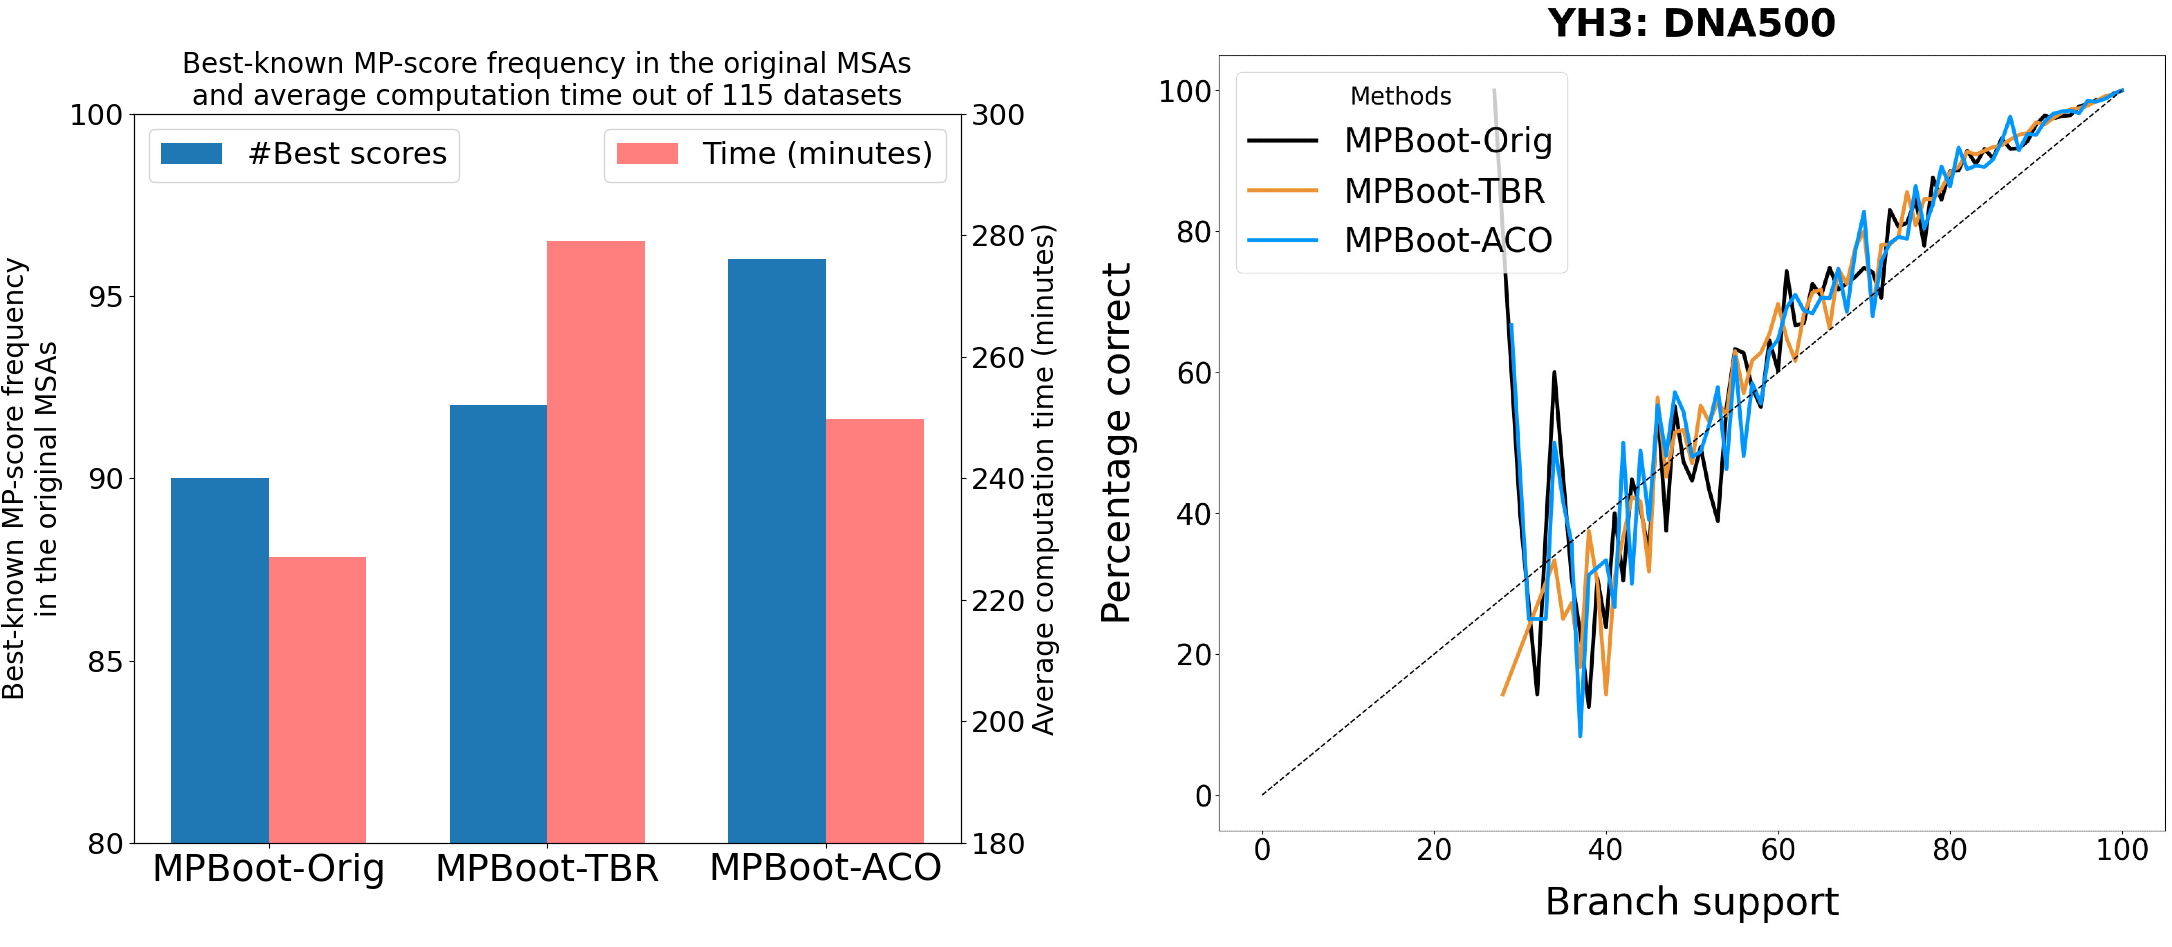
\includegraphics[width = 1\columnwidth]{./Figuras/results.png}
\caption{Evaluations result of MPBoot, MPBoot-TBR, and MPBoot-ACO}
\end{table}
\end{column}

\end{columns}
\end{block}
%
\end{column}
%
\end{columns}

\begin{columns}[t, onlytextwidth]
%
\begin{column}{0.49\textwidth}
%
\begin{block}{CONCLUSIONS}
\vspace{0.5cm}
\begin{itemize}
\item We have proposed the MPBoot-TBR (with two different search strategies) and the MPBoot-ACO algorithm.
\item The experimental results indicate that the performance in MP scores is improved with MPBoot-TBR and even further improved with MPBoot-ACO, while maintaining the same level of bootstrap accuracy as the original MPBoot. Moreover, MPBoot-ACO exhibits a faster processing time than MPBoot-TBR.
\item We have implemented the proposed algorithm based on open-source software MPBoot, available at Github for \href{https://github.com/HynDuf/mpboot/tree/Huynh_Tien_Dung}{MPBoot-TBR} and \href{https://github.com/HynDuf/mpboot/tree/ant-colony-optimization}{MPBoot-ACO}.
\end{itemize}
\end{block}
%https://www.overleaf.com/project/642e53668e325c8e22493e8a
\end{column}
%
\begin{column}{0.49\textwidth}
%
\begin{block}{RELATED PUBLICATION}
\vspace{0.5cm}
\begin{itemize}
    \item \footnotesize{T. D. Huynh, Q. T. Vu, V. D. Nguyen and D. T. Hoang, "Employing tree bisection and reconnection rearrangement for parsimony inference in MPBoot," \textbf{2022 14th International Conference on Knowledge and Systems Engineering (KSE)}, Nha Trang, Vietnam, 2022, pp. 1-6, Oct. 2022. ISSN 2694-4804. DOI: \url{https://doi.org/10.1109/KSE56063.2022.9953773}.}
\end{itemize}
\end{block}
\begin{block}{REFERENCES}
\vspace{0.5cm}
\printbibliography[heading = none]
\end{block}
%
\end{column}
%
\end{columns}

\vspace*{\stretch{20}}

\respnotice[Address]{E3 building, 144 Xuan Thuy road, Cau Giay district, Hanoi, Vietnam.}\\
\respnotice[Tel.]{+84-24-37547 461.}\\
\respnotice[Website]{http://www.vnu.edu.vn}

\vspace*{\baselineskip}

\end{frame}

%% Fim do documento
\end{document}
